\chapter{Half Wave Rectifier}
\vspace{-1cm}

%--------------------------AIM-----------------------------
\section{Aim}
\hspace{1cm}Single Phase Half Wave Uncontrolled and Controlled Rectifier

%--------------------------SOFTWARE USED-----------------------------
\section{Software Used}
\hspace{1cm}MATLAB R2020a
%-------------------------THEORY---------------------------
\section{Theory}
\hspace{\parindent}
A rectifier is a device that converts alternating current (AC) to direct
current (DC). It is done by using a diode or a group of diodes.
A half wave rectifier is defined as a type of rectifier that only allows
one half-cycle of an AC voltage waveform to pass, blocking the other
half-cycle. Half-wave rectifiers are used to convert AC voltage to DC
voltage, and only require a single diode to construct.

\hspace{\parindent}
\textbf{Single Phase Half Wave Uncontrolled Rectifier:}
This rectifier comprises of an AC source, a diode and a load. The
diode gets forward biased during the positive half cycle of the AC
source, and the circuit conducts. During the negative half cycle, the
diode becomes reverse biased and blocks current.

\hspace{\parindent}
\textbf{Single Phase Half Wave Controlled Rectifier:}
This rectifier comprises of an AC source, a Thyristor/SCR and a
load. The key difference here, is the presence of the thyristor/SCR,
which conducts only when gate pulses at a firing angle $ \alpha $ are applied
to it. The SCR automatically turns off when its voltage is reverse
biased for a period longer than the SCR turn off time and its current
falls below holding current.


% \vspace{1cm}

%----------------------Theoretical Calculations----------------------
\section{Theoretical Calculations}
\hspace{\parindent}
For an R load, average output voltage and current for a controlled
half wave rectifier are given by:

$$
    V_{o,avg} =
    V_{phase}
    \sqrt{2(1 + cos\alpha)2\pi} =
    V_m(1 + cos\alpha)
    2\pi
$$
$$
    I_{o,avg} =
    V_oR
$$

Where $ \alpha $ is the firing angle of the thyristor. For uncontrolled recti-
fiers, the thyristor is replaced by a diode, and $ \alpha $ = 0.

For a single phase half wave uncontrolled rectifier


%-----------------------circuit 1--------------------------
\section{Single Phase Half Wave Uncontrolled Rectifier with R load}

\subsection{Circuit used for simulation}

% figure that is centered on the page
\begin{figure}[h]
    \centering
    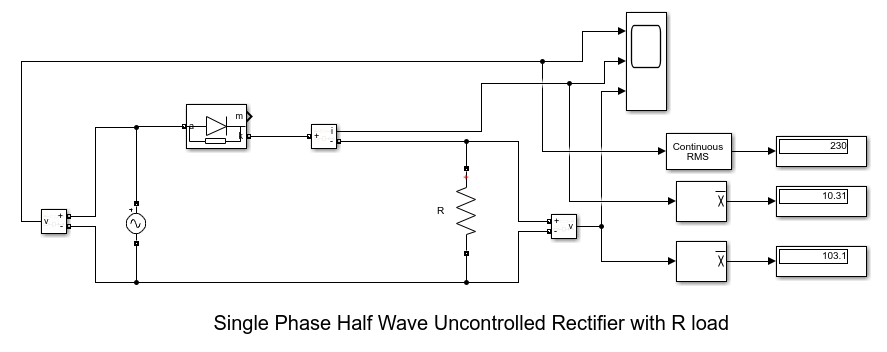
\includegraphics[width=0.7\textwidth]{images/experiment-1/circuit-diagram-simulation-01.png}
    \caption{Circuit used for simulation}
    \label{Fig_simulation_circuit_single-phase-half-wave-uncontrolled-rectifier-with-R-load}
\end{figure}

\subsection{Components Required}

\begin{table}[h]
    \renewcommand{\arraystretch}{1.3}
    \label{table_components_required_circuit_1}
    \centering
    \begin{tabular}{|c|c|c|c|}
        \hline
        Sr. No & Parameters                     & Ratings            & Quantity \\
        \hline
        \hline
        1      & AC Single Phase Voltage Source & 230V ($ V_{rms} $) & 1        \\
        \hline
        2      & Resistor                       & 10$ \Omega $       & 1        \\
        \hline
        3      & Diode                          & -                  & 1        \\
        \hline
        4      & Voltmeter                      & -                  & 2        \\
        \hline
        5      & Ammeter                        & -                  & 1        \\
        \hline
    \end{tabular}
    \caption{Components for Single Phase Half Wave Uncontrolled Rectifier with R load}

\end{table}




\subsection{Observations}

\begin{table}[h]
    \renewcommand{\arraystretch}{1.3}
    \label{table_observation_circuit_1}
    \centering
    \begin{tabular}{|c|c|c|}
        \hline
        Parameters                              & Theoretical Values & Simulation Values \\
        \hline
        \hline
        AC Input Voltage ($ V_{in,rms} $)       & 230V               & 230V              \\
        \hline
        Output Average Voltage ($ V_{o,avg} $)  & 103.53V            & 103.1V            \\
        \hline
        Output Average Current ($ I_{o,avg}  $) & 10.35A             & 10.31A            \\
        \hline
        AC Input Power ($ P_{AC}  $)            & 2389.5 W           & 2372 W            \\
        \hline
        DC Input Power ($ P_{DC}  $)            & 1071.53 W          & 1063 W            \\
        \hline
        Efficiency (\%)                         & 44.84              & 44.84             \\
        \hline
    \end{tabular}
    \caption{Observations for Single Phase Half Wave Uncontrolled Rectifier with R load}

\end{table}


The simulated values closely match the theoretical values, suggesting that the circuit is functioning correctly. Since the load is resistive, the output current is in phase with the output voltage. The output voltage and current waveforms indicate that the diode is forward-biased during the positive half-cycle of the AC source.

\pagebreak

\subsection{Resultant Waveforms}

% figure that is centered on the page
\begin{figure}[h]
    \centering
    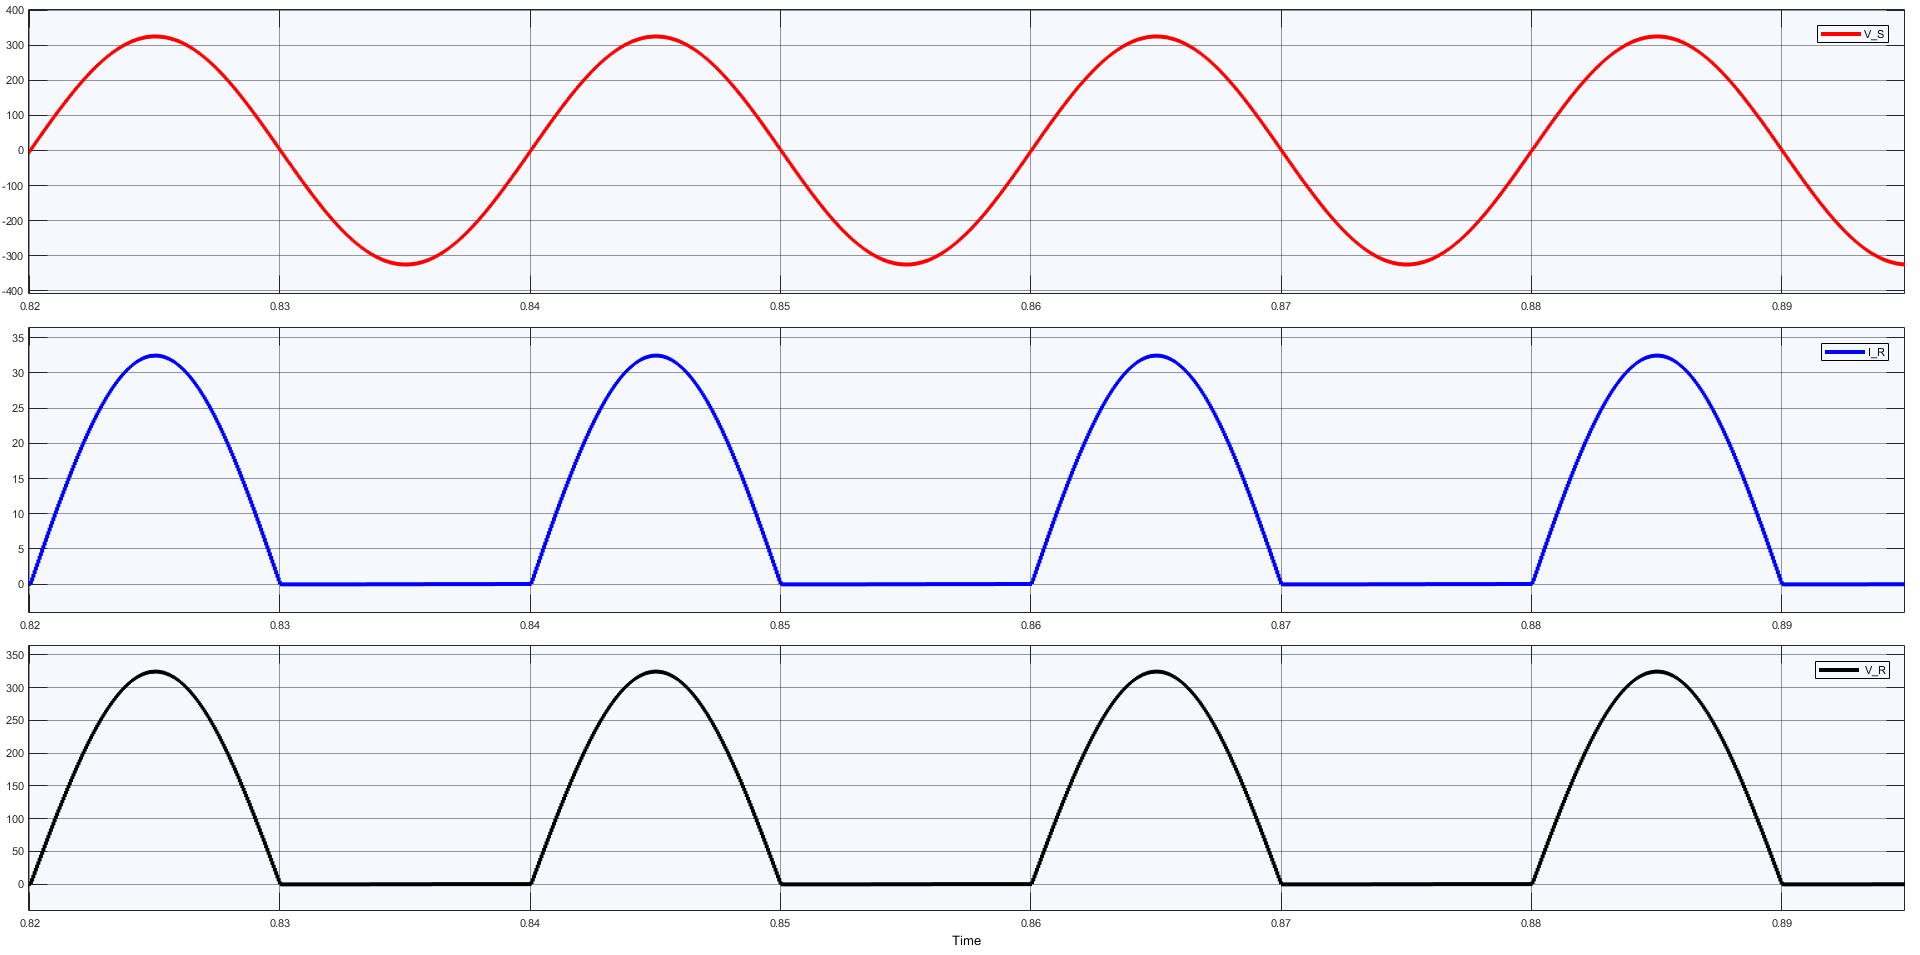
\includegraphics[width=1\textwidth]{images/experiment-1/circuit-scope-simulation-01.png}
    \caption{Scope Waveforms for Single Phase Half Wave Uncontrolled Rectifier with R load waveforms}
    \label{Fig_waveform_single-phase-half-wave-uncontrolled-rectifier-with-R-load}
\end{figure}

\pagebreak

%-----------------------circuit 2--------------------------
\section{Single Phase Half Wave Uncontrolled Rectifier with RL load}

\subsection{Circuit used for simulation}

% figure that is centered on the page
\begin{figure}[h]
    \centering
    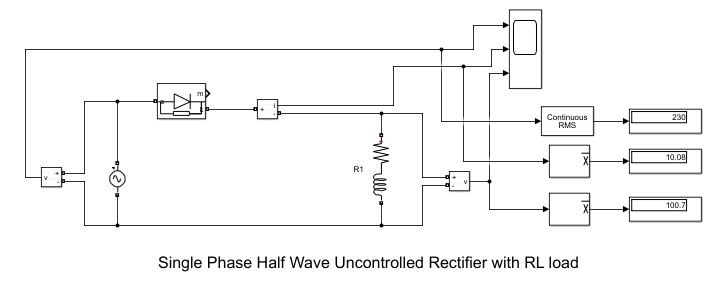
\includegraphics[width=0.7\textwidth]{images/experiment-1/circuit-diagram-simulation-02.png}
    \caption{Circuit used for simulation}
    \label{Fig_simulation_circuit_single-phase-half-wave-uncontrolled-rectifier-with-RL-load}
\end{figure}

\subsection{Components Required}

\begin{table}[h]
    \renewcommand{\arraystretch}{1.3}
    \label{table_components_required_circuit_2}
    \centering
    \begin{tabular}{|c|c|c|c|}
        \hline
        Sr. No & Parameters                     & Ratings            & Quantity \\
        \hline
        \hline
        1      & AC Single Phase Voltage Source & 230V ($ V_{rms} $) & 1        \\
        \hline
        2      & Resistor                       & 10$ \Omega $       & 1        \\
        \hline
        3      & Inductor                       & 10mH               & 1        \\
        \hline
        4      & Diode                          & -                  & 1        \\
        \hline
        5      & Voltmeter                      & -                  & 2        \\
        \hline
        6      & Ammeter                        & -                  & 1        \\
        \hline
    \end{tabular}
    \caption{Components for Single Phase Half Wave Uncontrolled Rectifier with RL load}
\end{table}


\subsection{Observations}

\begin{table}[h]
    \renewcommand{\arraystretch}{1.3}
    \label{table_observation_2}
    \centering
    \begin{tabular}{|c|c|c|}
        \hline
        Parameters                              & Theoretical Values & Simulation Values \\
        \hline
        \hline
        AC Input Voltage ($ V_{in,rms} $)       & 230V               & 230V              \\
        \hline
        Output Average Voltage ($ V_{o,avg} $)  & 103.53V            & 100.8V            \\
        \hline
        Output Average Current ($ I_{o,avg}  $) & 10.35A             & 10.08A            \\
        \hline
        AC Input Power ($ P_{AC} $)             & 2389.5 (W)         & 2318 (W)          \\
        \hline
        DC Input Power ($ P_{DC} $)             & 1071.53 (W)        & 1017 (W)          \\
        \hline
        Efficiency (\%)                         & 44.84              & 43.84             \\
        \hline
    \end{tabular}
    \caption{Observations for Single Phase Half Wave Uncontrolled Rectifier with RL load}

\end{table}


The circuit's simulated values are in good agreement with the theoretical values. Nonetheless, the load contains an inductive component that causes the output current to lag behind the output voltage. This delay results in the diode conducting until the output current reaches zero, which causes the output voltage to become negative during this period. Once the output current reaches zero, the diode stops conducting, and the output voltage returns to zero.
The efficiency of uncontrolled rectifier with RL load is 44.84\%.
\pagebreak


\subsection{Resultant Waveforms}

% figure that is centered on the page
\begin{figure}[h]
    \centering
    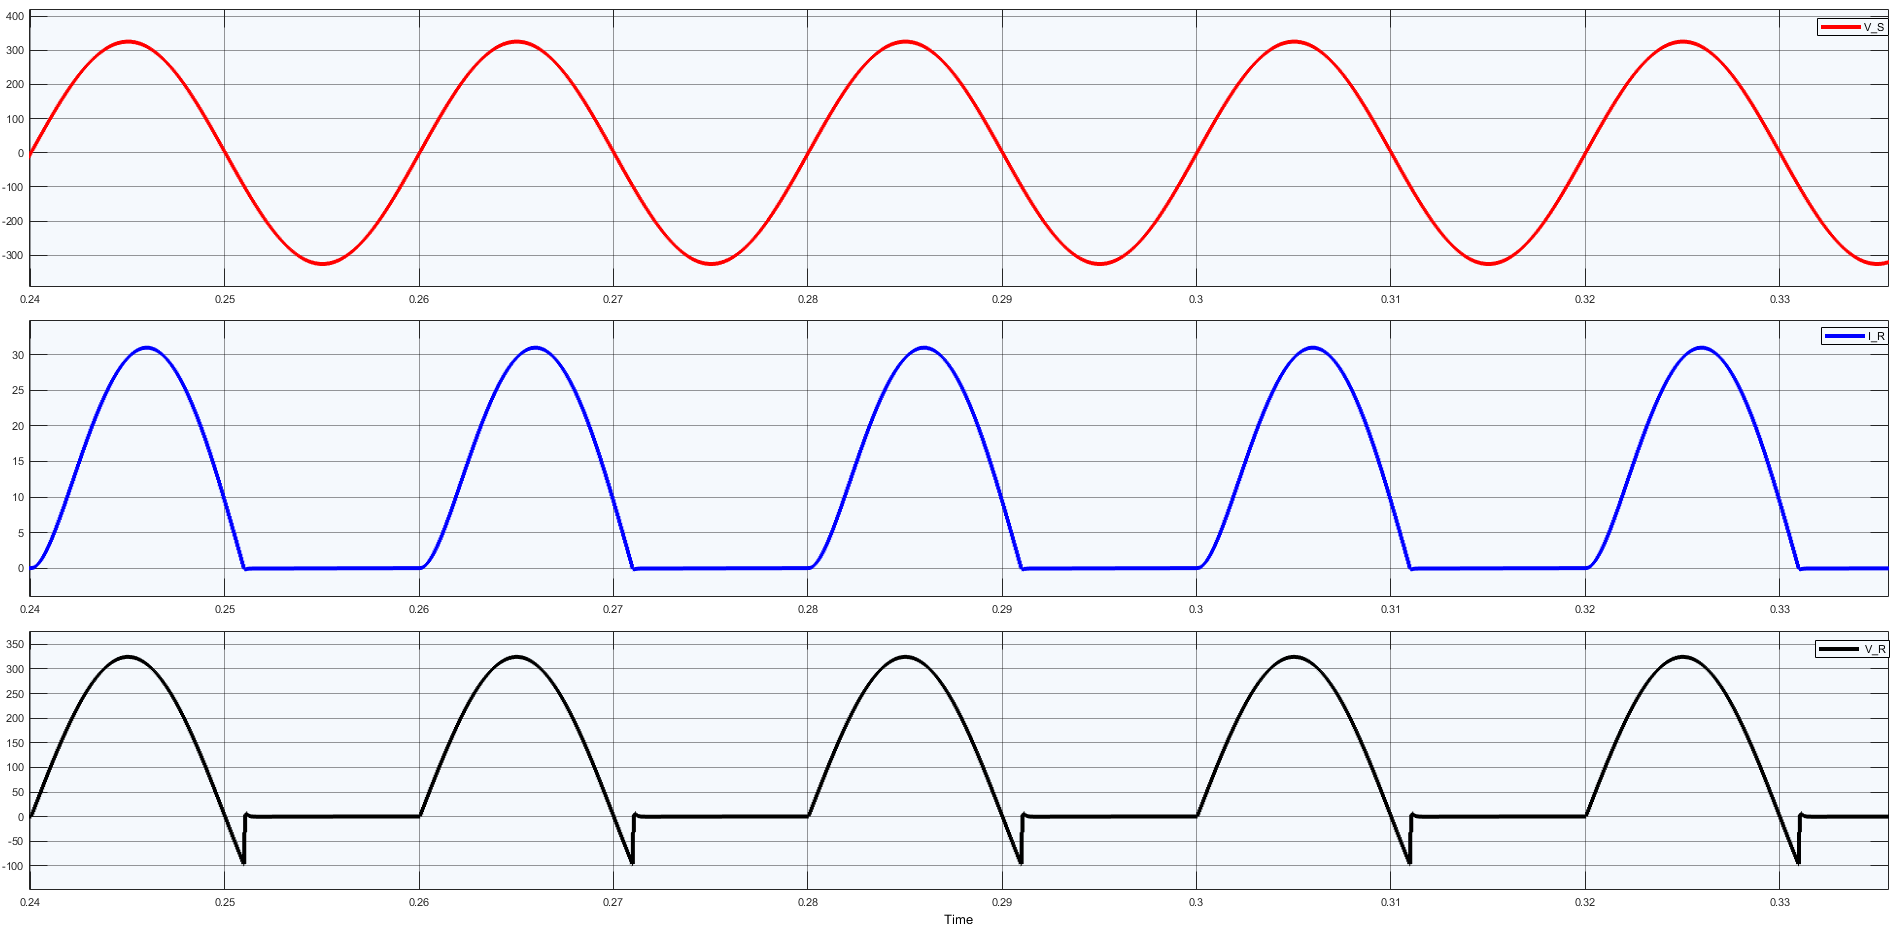
\includegraphics[width=1\textwidth]{images/experiment-1/circuit-scope-simulation-02.png}
    \caption{Scope Waveforms for Single Phase Half Wave Uncontrolled Rectifier with RL load}
    \label{Fig_waveform_single-phase-half-wave-uncontrolled-rectifier-with-RL-load}
\end{figure}

\pagebreak

\section{Single Phase Half Wave Uncontrolled Rectifier with RL load and Freewheeling Diode}

\subsection{Circuit used for simulation}

% figure that is centered on the page
\begin{figure}[h]
    \centering
    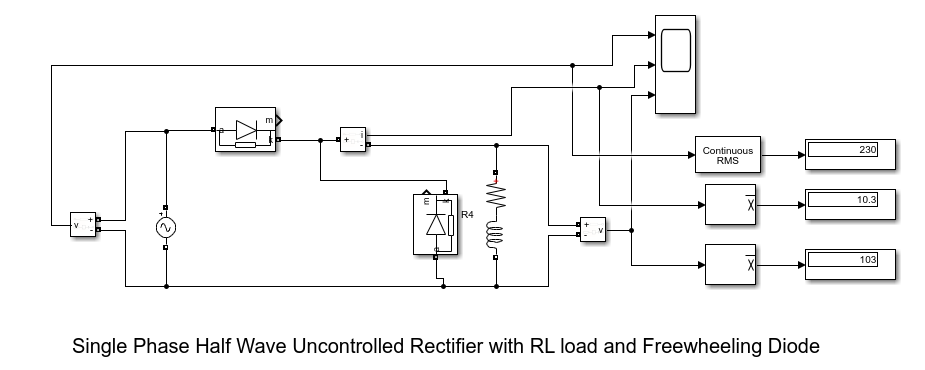
\includegraphics[width=0.7\textwidth]{images/experiment-1/circuit-diagram-simulation-03.png}
    \caption{Circuit used for simulation}
    \label{Fig_simulation_circuit_single-phase-half-wave-uncontrolled-rectifier-with-RL-load-and-freewheeling-diode}
\end{figure}

\subsection{Components Required}

\begin{table}[h]
    \renewcommand{\arraystretch}{1.3}
    \label{table_components_required_circuit_3}
    \centering
    \begin{tabular}{|c|c|c|c|}
        \hline
        Sr. No & Parameters                     & Ratings            & Quantity \\
        \hline
        \hline
        1      & AC Single Phase Voltage Source & 230V ($ V_{rms} $) & 1        \\
        \hline
        2      & Resistor                       & 10$ \Omega $       & 1        \\
        \hline
        3      & Inductor                       & 10mH               & 1        \\
        \hline
        4      & Diode                          & -                  & 1        \\
        \hline
        5      & Voltmeter                      & -                  & 2        \\
        \hline
        6      & Ammeter                        & -                  & 1        \\
        \hline
    \end{tabular}
    \caption{Components for Single Phase Half Wave Uncontrolled Rectifier with RL load and Freewheeling Diode}
\end{table}


\subsection{Observations}

\begin{table}[h]
    \renewcommand{\arraystretch}{1.3}
    \label{table_observation_3}
    \centering
    \begin{tabular}{|c|c|c|}
        \hline
        Parameters                              & Theoretical Values & Simulation Values \\
        \hline
        \hline
        AC Input Voltage ($ V_{in,rms} $)       & 230V               & 230V              \\
        \hline
        Output Average Voltage ($ V_{o,avg} $)  & 103.53V            & 103V              \\
        \hline
        Output Average Current ($ I_{o,avg}  $) & 10.35A             & 10.3A             \\
        \hline
        AC Input Power ($ P_{AC}  $)            & 2389.5 (W)         & 2404 (W)          \\
        \hline
        DC Input Power ($ P_{DC}  $)            & 1071.53 (W)        & 1061 (W)          \\
        \hline
        Efficiency (\%)                         & 44.84              & 44.13              \\
        \hline
    \end{tabular}
    \caption{Observations for Single Phase Half Wave Uncontrolled Rectifier with RL load and Freewheeling Diode}

\end{table}



The simulated and calculated values demonstrate that the simulated output voltage is close to the calculated voltage, but the simulated output current varies from the calculated current. Additionally, the inclusion of the freewheeling diode causes the output current in the rectifier circuit to cut off abruptly when the source AC supply reaches zero volts, as the lagging current begins to flow through the freewheeling diode rather than the rectifier circuit.
The efficiency of uncontrolled rectifier with RL load with freewheeling diode is 44.13\%.

\pagebreak

\subsection{Resultant Waveforms}


% figure that is centered on the page
\begin{figure}[h]
    \centering
    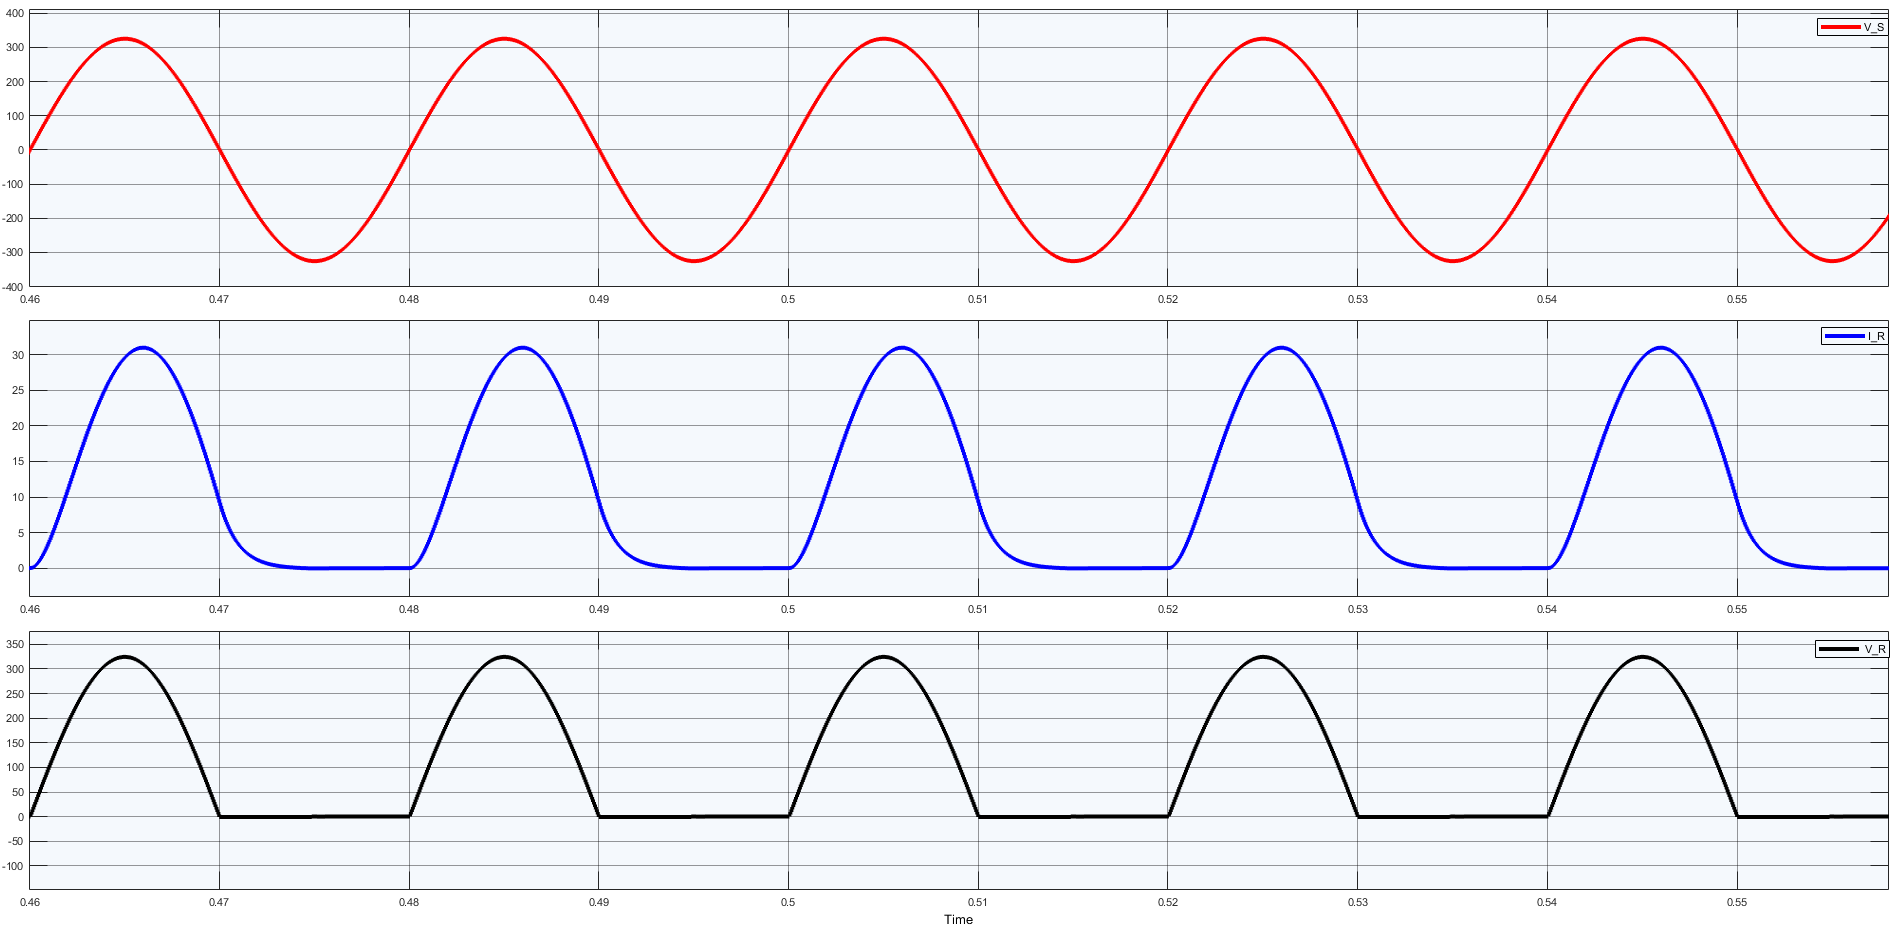
\includegraphics[width=1\textwidth]{images/experiment-1/circuit-scope-simulation-03.png}
    \caption{Scope Waveforms for Single Phase Half Wave Uncontrolled Rectifier with RL load and Freewheeling Diode}
    \label{Fig_waveform_single-phase-half-wave-uncontrolled-rectifier-with-RL-load-and-freewheeling-diode}
\end{figure}


\pagebreak





%-------------------------RESULTS---------------------------
\section{Results}
%------------SUB----------RESULTS---------------------------
\subsection{Theoretical Calculation}


\hspace{1.5cm} The resistance \textbf{R} in the circuit shown in Fig. 2.2 is considered as 20 $\Omega$, and the voltage (which is effectively the voltage across \textbf{R}) is considered as 50 V, 100 V, 150 V and 200 V in four steps as mentioned in the second column of Table-\ref{Table_simulation-result}. As per \textbf{Ohm's Law}, the current corresponding to all the four voltages are,
$$I=\frac{V}{R}=\frac{50}{20}= 2.5~A~~ (for~ V =50 V);~~~   = 5~A~~ (for~ V =100 V);~~~
    = 7.5~A~~ (for~ V =150 V);~~~= 10~A~~ (for~ V =200 V) $$


%------------SUB----------RESULTS---------------------------
\subsection{Simulation Results}
\hspace{1.5cm} The simulink file is run for 10 sec considering V=50 V, and and corresponding current seen in the display is noted in the fourth column of second row of Table-\ref{Table_simulation-result}. Similarly, all other three rows are filled.  Further, constantly varying ramp voltage is applied and the corresponding \textit{v-i} graph is plotted in Fig. \ref{Fig_v-i graph}.

\begin{minipage}{\textwidth}
    \begin{minipage}[b]{0.6\textwidth}
        \centering
        \begin{tabular}{|c|c|c|c|}
            \hline
            \multirow{2}{*}{Sl No} & \multirow{2}{*}{Applied Voltage (V) in Volts} & \multicolumn{2}{c|}{Current (I) through R in Amps}             \\
            \cline{3-4}
                                   &                                               & Theoretical                                        & Simulated \\
            \hline
            1                      & 50                                            & 5                                                  & 2.5       \\
            \hline
            2                      & 100                                           & 10                                                 & 5         \\
            \hline
            3                      & 150                                           & 15                                                 & 7.5       \\
            \hline
            4                      & 200                                           & 20                                                 & 10        \\
            \hline
        \end{tabular}
        \captionof{table}{Simulation Results}
        \label{Table_simulation-result}
    \end{minipage}
    \hfill

\end{minipage}

\section{Discussion}
\hspace{1.5cm} From the data of third and fourth column of Table-\ref{Table_simulation-result}, it is seen that the simulated values exactly matches with the corresponding theoretical numbers. Further, the simulated \textit{v-i} plot also matches with the theoretical\textit{v-i} plot (see Fig. ) of a resistance. The slope of the plot represents the resistance what is consider in the simulation. For example, consider the point at (100,5), and the slope of the line is $\frac{100-0}{5-0}=20$ and that is the value of resistance. It is also seen that the \textit{v-i} characteristics is same for sinusoidal applied voltage.

\section{Observation}
\subsection{For Simulation}
\begin{enumerate}
    \item Proper simulation step size has to be chosen fro the simulation. In case of sinusoidal forcing function, the step size is chosen to be $10^{-4}$ s.
\end{enumerate}
\subsection{For Real Experiment}
\begin{enumerate}
    \item There might be error in resistance value which results in slightly mismatch in the results.
    \item There might be a chance of error in readings due to analog instruments.
    \item There might be a chance of change in temperature of the resistance if the experiment is run for long time, which effects the experimental results.
\end{enumerate}

\section{Conclusion}
\hspace{1.5cm} Verification of Ohm's Law is done through simulation in Matlab/Simulink platform. The simulation is done considering constant DC voltage, variable ramp voltage and sinusoidal voltage. In each case, the theoretical and simulated results matches well.

\begin{thebibliography}{15}

    \bibitem{journal1} R.E. Higgs, K.G. Bemis, I.A. Watson and J.H. Wikel, “Experimental designs for selecting molecules from large chemical databases”, \textit{Journal of Chemical Information and Computer Sciences}, 37(5), 861-870, September 1997.

    \bibitem{conference1} N. Paivinen and T. Gronfors, “Minimum spanning tree clustering of EEG signals”, \textit{$6^{th}$ Nordic Signal Processing Symposium (NORSIG-2004)}, Finland, pp. 149-152, June 9-11, 2004.

\end{thebibliography}
\pagebreak

%==========================================================
%           CHAPTER : Verification of Kirchhoff’s Law 
%==========================================================
